\documentclass[a4paper,12pt,titlepage,oneside,openany]{book}
\usepackage[top=4cm,bottom=4cm,left=2cm,right=2cm]{geometry}
\usepackage[italian]{babel}
\usepackage[utf8]{inputenc}
\usepackage{amsmath,amssymb,amsfonts,amsthm,graphicx,mathrsfs,braket,float}
\usepackage[hidelinks]{hyperref}
\usepackage{bytefield}
\usepackage{multirow}
\usepackage{url}
\setcounter{secnumdepth}{4} 
\setcounter{tocdepth}{3}
\linespread{1.4}
\graphicspath{ {./Images/} }

\begin{document}
\clearpage
\thispagestyle{empty}
\begin{figure}
	\centering
	\vspace*{2cm}	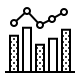
\includegraphics{logo.png}
	\label{fig:logo}
\end{figure}

\centerline{\rule{16cm}{0.2mm}}
\vspace*{2cm}
\centerline{\LARGE{Linear Regression Tool}}
\vspace*{2cm}
\centerline{\rule{8cm}{0.2mm}}\medskip
\centerline{Relazione progetto: Metodi matematici e statistici(6CFU)}
\centerline{\rule{8cm}{0.2mm}}
\vspace*{1.19cm}
\centerline{Pietro Biondi}
\vspace*{2cm}

\centerline{\rule{16cm}{0.2mm}}
\newpage
\thispagestyle{empty}
\tableofcontents
\thispagestyle{empty}
\newpage
\chapter*{Introduzione}
\addcontentsline{toc}{chapter}{Introduzione}
\markboth{Introduzione}{Introduzione} 
Al giorno d'oggi in giro per il web vi sono sempre più dati disponibili su cui poter effettuare delle statistiche interessanti. Attraverso l'uso di linguaggi di programmazione come Python / MATLAB è possibile manipolare i dati e ricavare tutte le statistiche che si desiderano.\\
Linear Regression Tool (LRT) consente di calcolare attributi e statistiche attraverso le funzioni disponibili in Python2.7, come:
\begin{itemize}
	\item[•] Regressione lineare (coefficienti m,q);
	\item[•] Covarianza
	\item[•] Coefficiente di Pearson.
\end{itemize}
A questo proposito, grazie al coefficiente di Pearson è possibile carpire se le due variabili sono correlate o meno.
\chapter{Regressione Lineare}
La regressione formalizza e risolve il problema di una relazione funzionale tra variabili misurate sulla base di dati campionari estratti da un'ipotetica popolazione infinita.
Originariamente Galton utilizzava il termine come sinonimo di correlazione, tutta via oggi in statistica l'analisi della regressione è associata alla risoluzione del modello lineare. Per la loro versatilità, le tecniche della regressione lineare trovano impiego nel campo delle scienze applicate come: chimica, geologia, biologia, fisica, ingegneria, medicina. Inoltre la regressione lineare viene utilizzata nelle scienze sociali come: economia, linguistica, psicologia, sociologia.\par
\noindent \\
Più formalmente in statistica la regressione lineare rappresenta un metodo di stima del valore atteso condizionato di una variabile dipendete, {\itshape Y}, dati i valori altre variabili indipendeti, \begin{math} X_{1},...,X_{k} \end{math}.
La retta di regressione si ottiene applicando il metodo dei minimi quarati.
Il modello di regressione lineare è quindi:
\begin{center}
  \begin{math}
    Y_{i}=\beta_{0}+\beta_{1}X_{i}+u_{i}
  \end{math}
\end{center}
\newpage
Dove:
\begin{itemize}
  \item i varia tra le osservazioni \begin{math} i=1,...,n \end{math} .
  \item \begin{math} Y_{i} \end{math} è la variabile dipendente.
  \item \begin{math} X_{i} \end{math}  è la variabile indipendente. 
  \item \begin{math} \beta_{0}+\beta_{1}X \end{math} è la retta di regressione o funzione di regressione della popolazione.
  \item \begin{math} \beta_{0} \end{math} è l'intercetta della retta di regressione della popolazione, ovvero il punto dove la retta incontra l'asse delle ordinate.
  \item \begin{math} \beta_{1} \end{math} è il coefficiente angolare della retta di regressione della popolazione, esso indica quando varia la y la variare di x.
  \item \begin{math} u_{i} \end{math} è l'errore statistico.
\end{itemize}
\begin{figure}[H]
	\centering	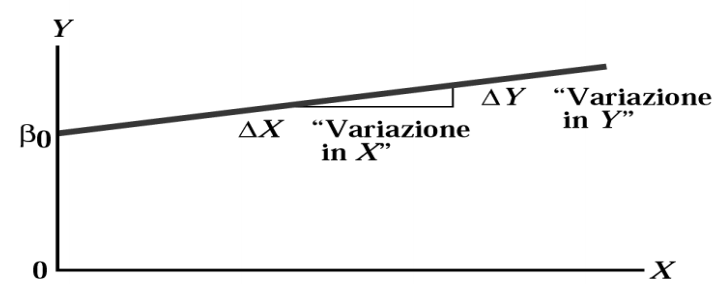
\includegraphics[scale=0.5]{regression.png}
	\label{fig:regression}
\end{figure}
L'inclinazione 
\begin{math}
	\beta_{1}
\end{math}
indica come varia Y in corrispondenza di una variazione unitaria di X. Il segno di \begin{math} \beta_{1} \end{math} indica se la relazione lineare è positiva o negativa.
L’intercetta \begin{math} \beta_{0} \end{math} corrisponde al valore medio di Y quando X è uguale a 0.
Per ogni osservazione campionaria si dispone di una determinazione Y e di K determinazioni non dipendenti (non stocastiche) \begin{math} X_{1},X_{2},...,X_{k} \end{math}. Si cerca quindi una relazione di tipo lineare tra la variabile Y e le k variabili deterministiche. Per cui possiamo dire che la regressione viene utilizzata per costruire un modello attraverso cui prevedere i valori di una variabile dipendente o risposta (quantitativa) a partire dai valori di una o più variabili indipendenti o esplicative.
\chapter{Funzionamento}
L’applicazione è interamente sviluppata in Python 2.7 per il funzionamento è necessario importare delle librerie, nello specifico:
\begin{itemize}
	\item[•] \textit{Numpy} (libreria per la computazione scientifica che include la possibilità di effettuare operazioni su array e matrici).
	\item[•] \textit{Matplotlib} (libreria per la creazione di grafici 2D)
	\item[•] \textit{SciPy} (libreria di algoritmi, strumenti matematici e strutture dati. Contiene moduli per l’ottimizzazione per algebra lineare, l’integrazione, FFT, elaborazione di segnali)
	\item[•] \textit{Sklearn} (libreria per il machine learning che contiene algoritmi di classificazione regressione e clustering. Sklearn è stata progettata per operare con Numpy e SciPy)
	\item[•] \textit{Statistics} (libreria che fornisce metodi per calcolo statistico)
\end{itemize}
\begin{figure}[H]
	\centering	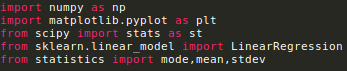
\includegraphics{importlib.png}
	\label{fig:importlib}
	\caption{Import librerie}
\end{figure}
\newpage
Definizione e inizializzazione array:
\begin{figure}[H]
	\centering	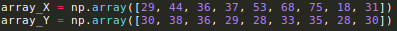
\includegraphics{array.png}
	\label{fig:array}
\end{figure}
Inizializzazione del regressore, allenamento e calcolo dati:
\begin{figure}[H]
	\centering	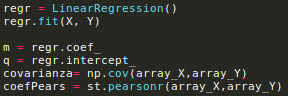
\includegraphics{regressioncode.png}
	\label{fig:regressioncode}
\end{figure}
Plotting dei dati (grafico):
\begin{figure}[H]
	\centering	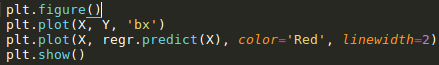
\includegraphics{plotcode.png}
	\label{fig:plotcode}
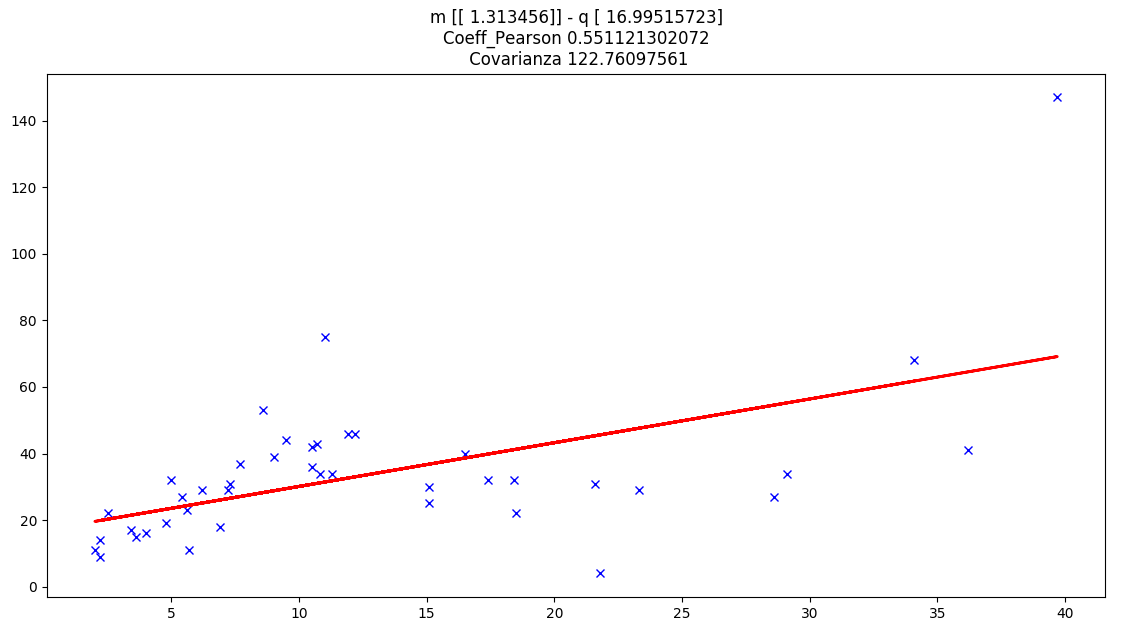
\includegraphics[scale=0.4]{plotgraph.png}
	\label{fig:plotgraph}
\end{figure}
\newpage
\paragraph*{Spiegazione}
L’applicazione richiede l’inserimento dei dati tramite array di numpy come visualizzato nel punto precedente.
Una volta inseriti i dati, l’oggetto \textit{LinearRegression()} di Sklearn verrà allenato con i rispettivi parametri X , Y. Successivamente sarà possibile ottenere il coefficiente angolare (m) e il termine noto (q).
Avendo a disposizione i due array, è inoltre possibile ottenere altri dati statistici come covarianza e coefficiente di Pearson, che mostrerà la correlazione tra i due dati.
\chapter{Risultati e conclusioni}
Avendo inserito come input gli array X e Y, rispettivamente pari a :\\
X = np.array([6.2, 9.5, 10.5, 7.7, 8.6, 34.1, 11, 6.9, 7.3, 15.1, 29.1, 2.2, 5.7, 2, 2.5, 4, 5.4, 2.2, 7.2, 15.1, 16.5, 18.4, 36.2, 39.7, 18.5, 23.3, 12.2, 5.6, 21.8, 21.6, 9, 3.6, 5, 28.6, 17.4, 11.3, 3.4, 11.9, 10.5, 10.7, 10.8, 4.8])
\\
Y = np.array([29, 44, 36, 37, 53, 68, 75, 18, 31, 25, 34, 14, 11, 11, 22, 16, 27, 9, 29, 30, 40, 32, 41, 147, 22, 29, 46, 23, 4, 31, 39, 15, 32, 27, 32, 34, 17, 46, 42, 43, 34, 19])\\
Abbiamo effettuato delle operazioni su essi.
Tramite le varie librerie abbiamo calcolato: regressione lineare, covarianza, coefficiente di Pearson, coefficiente angolare (m) e termine noto (q).
Nell’immagine sottostante vengono riportati i risultati calcolati tramite l’applicazione in Python 2.7
\begin{figure}[H]
	\centering	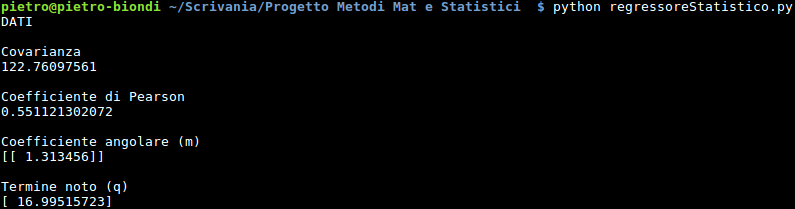
\includegraphics[scale=0.6]{risultati.png}
	\label{fig:risultati}
\end{figure}
\newpage
\paragraph*{Conclusioni}
Nella pratica si distinguono vari "tipi" di correlazione.
\begin{itemize}
	\item[•] Se 
	\begin{math}
		\rho_{XY}>0
	\end{math}, le variabili X e Y si dicono direttamente correlate, oppure correlate positivamente;
	\item[•] Se 
	\begin{math}
		\rho_{XY}=0
	\end{math}, le variabili X e Y si dicono incorrelate;
		\item[•] Se 
	\begin{math}
		\rho_{XY}<0
	\end{math}, le variabili X e Y si dicono inversamente correlate, oppure correlate negativamente.
\end{itemize}
Inoltre per la correlazione diretta (e analogamente per quella inversa) si distingue:
\begin{itemize}
	\item[•] Se 
	\begin{math}
		0<\rho_{XY}<0,3
	\end{math}, si ha correlazione debole;
	\item[•] Se 
	\begin{math}
		0,3<\rho_{XY}<0,7
	\end{math}, si ha correlazione moderata;
	\item[•] Se 
	\begin{math}
		\rho_{XY}>0,7
	\end{math}, si ha correlazione forte;
\end{itemize}
Avendo ottenuto un coefficiente di Pearson pari a 0.55, possiamo concludere che le due variabili X e Y sono correlate positivamente.
Inoltre possiamo affermare che si ha una correlazione moderata tra di esse poiché 
\begin{math}
	\rho_{xy}
\end{math} 
è compreso tra 0.3 e 0.7.
\chapter*{Sitografia}
\addcontentsline{toc}{chapter}{Sitografia}
\markboth{Sitografia}{Sitografia}
\begin{enumerate}
	
	\item Dataset,\\ \textit{ \tiny \url{http://college.cengage.com/mathematics/brase/understandable_statistics/7e/students/datasets/slr/frames/frame.html}}
		
	\item Regressione Lineare,\\ \textit{ \scriptsize \url{https://it.wikipedia.org/wiki/Regressione_lineare}}
				
		
	\item Coefficiente di Pearson,\\ \textit{\scriptsize \url{https://it.wikipedia.org/wiki/Indice_di_correlazione_di_Pearson}}
	
	\item Numpy,\\ \textit{\scriptsize \url{http://www.numpy.org/}}

	\item Matplotlib,\\ \textit{\scriptsize \url{http://matplotlib.org/}}

	\item SciPy,\\ \textit{\scriptsize \url{https://www.scipy.org/}}
	
	\item Sklearn,\\ \textit{\scriptsize \url{http://scikit-learn.org/stable/}}
	
	\item Statistics,\\ \textit{\scriptsize \url{https://docs.python.org/3/library/statistics.html}}
	
	
	
\end{enumerate}
\end{document}